\documentclass[journal,12pt,twocolumn]{IEEEtran}
\usepackage[utf8]{inputenc}
 
\usepackage{tfrupee}
\usepackage{enumitem}
\usepackage{amsmath}
\usepackage{amssymb}
\usepackage{graphicx}

\begin{document}

\newcommand{\myvec}[1]{\ensuremath{\begin{pmatrix}#1\end{pmatrix}}}

\let\vec\mathbf


\title{Assignment 2}
\author{\textbf{Himanshu Kumar Gupta (AI21BTECH11012)}}
\maketitle
\date {March 2022}


\textbf{\textit{Problem 1(viii), ICSE 12 2019:}}

Using L’Hospital’s Rule, evaluate:

 $\lim{x\to0} \frac{8^x-4^x}{4x}$

\textbf{\textit{Solution:}}

we know that,

if there is a function $f(x)=\frac{g(x)}{h(x)}$

then by L’Hospital’s Rule 
\begin{align}
\lim{x\to x_0} f(x)&=\lim{x\to x_0} \frac{g(x)}{h(x)}  \\
\label{eq:2}
&=\lim{x\to x_0} \frac{g'(x)}{h'(x)}
\end{align}
so,by equation \eqref{eq:2},
\begin{align}
\lim{x\to0} \frac{8^x-4^x}{4x}&=\lim{x\to0}
 \frac{\frac{\mathrm{d}(8^x-4^x)}{\mathrm{d}x}}{\frac{\mathrm{d}(4x)}{\mathrm{d}x}} \\
&=\lim{x\to0}\frac{8^x\log{8}-4^x\log{4}}{4}
\end{align}
Now,putting value of x=0,we get
\begin{align}
&=\frac{\log{8}-\log{4}}{4}       \\
&=\frac{\log{2}}{4}
\end{align}

\begin{figure}[htb!]
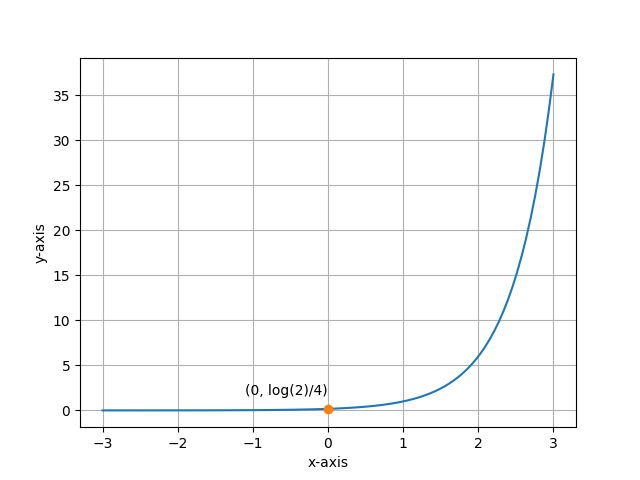
\includegraphics[width=0.60\textwidth]{figures/Figure_2.png}
\caption{graph representing the given curve and limiting point}
\end{figure}
\end{document}